Es gibt einige verschiedene Arbeiten die sich um das Thema Cross-Plattform beziehungsweise Multi-Plattform Entwicklung drehen. Die meisten Arbeiten sind dabei Veröffentlichungen im Rahmen von Konferenzen oder andere Wissenschaftliche Arbeiten. Im folgenden sollen einige vorgestellt werden und darauf eingegangen werden, was sie von dieser Arbeit unterscheidet.


\begin{figure}[ht]
  \centering
  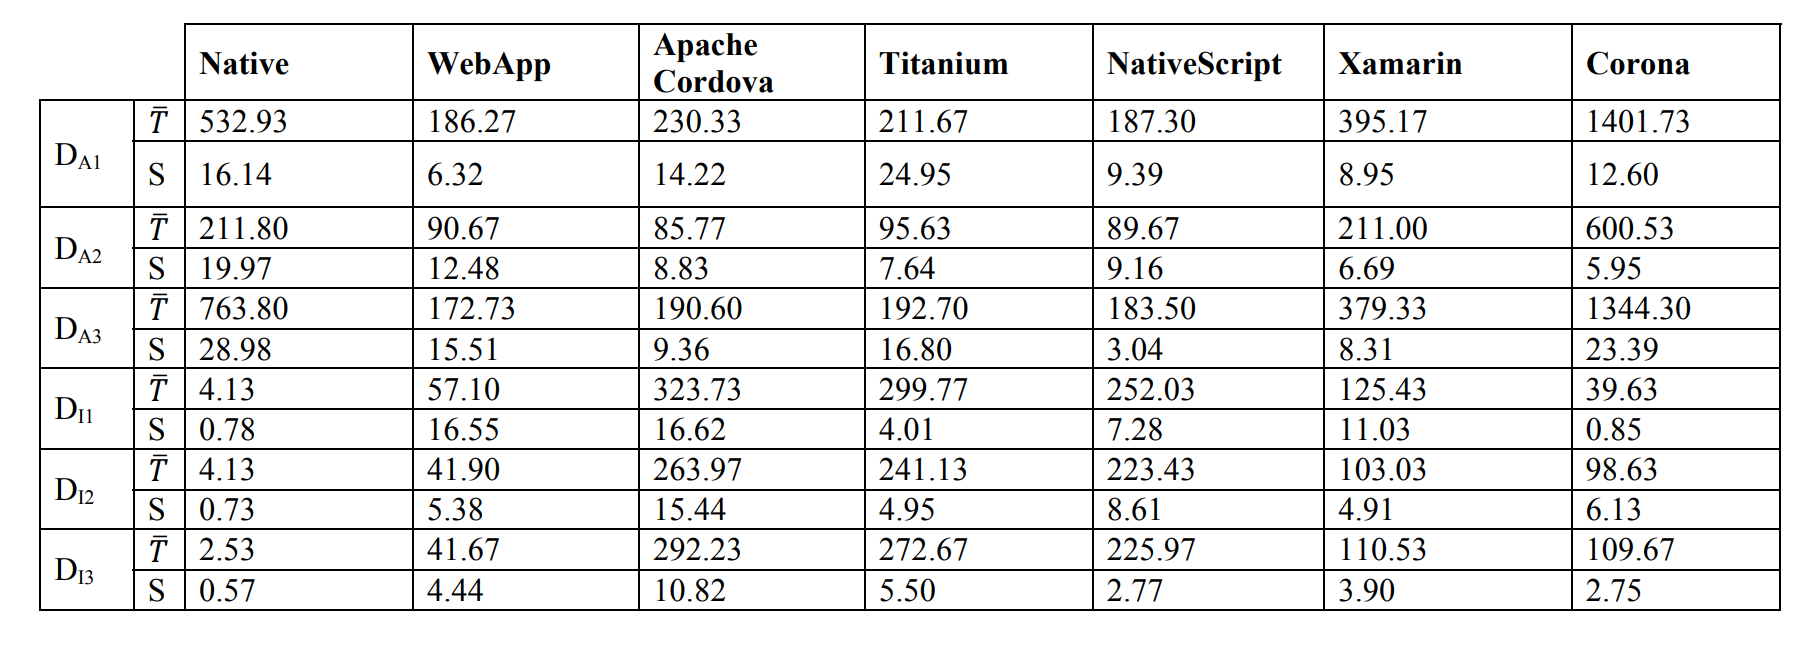
\includegraphics[width=\textwidth,keepaspectratio]{images/IEEE_Delia_Al.png}
  \caption{Ergebnisstabelle der Performancemessungen von Delia et al \cite{IEEE_development_classes}}
  \label{fig:result_table_IEEE_related_work}
\end{figure}

Die meisten Arbeiten drehen sich um den Faktor Performance. Hier gibt es viele unterschiedliche Untersuchungen. Delia et al \cite{IEEE_development_classes} etwa testete diese anhand von komplexen mathematischen Berechnungen und zeichnet dabei die verstrichene Zeit für iOS und Android auf. Dabei berechneten sie außerdem die Standardabweichung um zu untersuchen, wie gestreut die Ergebnisse sind. In Abbildung \ref{fig:result_table_IEEE_related_work} können diese betrachtet werden. Dabei stellte sie zwar einen Performance Unterschied zwischen Android und iOS fest, dieser ist jedoch ihrer Meinung nach, eher auf die unterschiedliche Hardware der Testgeräte zurückzuführen. Sie konnten aber insgesamt eine gute Performance von Web Applikationen feststellen. Die nativen Applikationen schnitten besonders unter Android deutlich schlechter ab als ein Großteil der restlichen Untersuchten Ansätze, jedoch auf iOS war dieser Ansatz bei ihnen der am besten performende.

In dieser Arbeit werden alle Tests auf einem Gerät durchgeführt um eine Vergleichbarkeit zu erlangen. Außerdem wird die Arbeit lediglich auf Android beschränkt, um mehr Fokus auf die unterschiedlichen Ansätze als auf die Unterschiede zwischen den Plattformen einzugehen. Außerdem werden in der Arbeit neben Performance viele weitere Faktoren untersucht. 
 
Denko et al \cite{Denko_performance} vergleichen nicht nur die verbrauchte Zeit für mathematische Berechnungen sondern analysieren zusätzlich die Auslastung der Geräte während verschiedenen Aufgaben und die Appgröße der kompilierten Apps. Die jeweiligen Parameter vergleichen sie dabei anhand drei Unterschiedlicher Geräte. Dabei konnten sie im am Ende keine eindeutige bessere Methode identifizieren, da oft je nach untersuchten Aspekt, ein anderer Ansatz besser war als ein anderer, dies aber bei einem anderen Faktor wieder vertauscht sein könnte. So war etwa bei der Ausführung von Algorithmen die Native Implementierung die schnellste, während Flutter hier eher als einer der schlechtesten abschnitt. Bei der Nutzung der CPU oder der Generationszeit einer compilierten Anwendung war Flutter dafür wieder besser als die native Android Implementierung. Sie kommen daher auf den Schluss, dass kein Ansatz in Sachen Performance der beste ist und deswegen eher andere Faktoren betrachtet werden müssen um eine fundierte Entscheidung zu treffen.

Wie auch in dieser Arbeit geplant, wurden hier zwar einige weitere Aspekte der Entwicklung in den Vergleich mit einbezogen, jedoch soll in dieser Arbeit die anderen Aspekte eine weit größere Rolle spielen, denn wie dieses Paper zeigt, kann anhand der Performance keine eindeutige Entscheidung getroffen werden.

In der Arbeit von  Andersson \cite{Andersson_2022} vergleicht er die Performanceunterschiede zwischen einer nativ entwickelten Android App und einer Cross-Plattform-App, die mit dem Flutter Framework geschrieben wurde. Dabei untersuchte er 6 verschiedene Funktionalitäten, die in vielen Apps vorkommen, so etwa Animationen, unendliche Listen oder auch Datenbankoperationen. Diese Funktionalität testete er und zeichnete dabei neben der Ausführungszeit auch die CPU und Speicherauslastung des Gerätes auf. Das Ergebnis war, dass auch er keinen eindeutig besseren Ansatz finden konnte, so war in seinem Vergleich Flutter deutlich schneller und Ressourcenschonender bei der Decodierung von Dateien. Dafür zeigte sein Test auch eine deutlich schlechtere Performance bei Animationen im Gegensatz zu der nativen Implementierung. Seine Schlussfolgerung ist dabei, dass Flutter Apps und dementsprechend Cross-Plattform Frameworks keine schlechtere Performance als native haben, es jedoch auf den genauen Anwendungsfall ankommt, welches Framework eine bessere Performance aufweist.

Auch in der Arbeit von Andersson wird wieder eine ähnliche Performance der untersuchten Technologien festgestellt, daher sollen in der folgenden Arbeit, wie bereits erwähnt, mehr Faktoren einbezogen werden. 

\begin{figure}[ht]
  \centering
  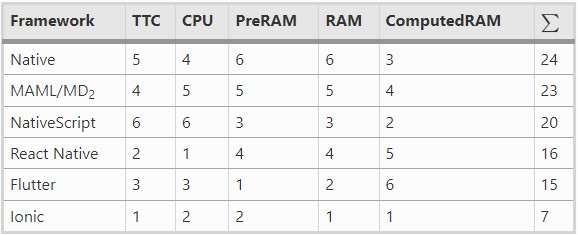
\includegraphics[width=10cm,keepaspectratio]{images/Biorn-Hansen_Result_table.jpg}
  \caption{Ergebnisstabelle der Untersuchung von Biørn-Hansen et al \cite{BirnHansen.2020}}
  \label{fig:result_table_Biorn}
\end{figure}

Biørn-Hansen et al \cite{BirnHansen.2020} konzentrieren sich in ihrer Untersuchung vor allem auf die Nutzung Plattformspezifischer Schnittstellen, wie etwa der Geo-Daten oder Kontakte \ac{API}. Die Untersuchten Maße sind dabei neben der Auslastung der Geräte vor allem die Zeit, bis eine Aufgabe abgeschlossen ist. Bei ihrer Auswertung der 5 Kriterien gewichteten sie jeden, der 6 implementierten Ansätzen, anhand einer Zahl von 1 - 6, wobei 6 die Implementierung bekommt, die am besten in diesem Bereich abgeschlossen hat und 1, die die schlechtesten Ergebnisse lieferte. Danach wurden die einzelnen erreichten Punkte zusammengerechnet und die Implementierung mit der höchsten Punktzahl ist die, die in ihrem Vergleich am besten abgeschlossen hat. Wie in Abbildung \ref{fig:result_table_Biorn} zu sehen ist, erreichte Nativ dabei eine Punktzahl von 24 und somit den 1. Platz in ihrer Auswertung. Das Cross-Plattform Framework Flutter hingegen landete auf dem vorletzten Platz mit gerade einmal 15 Punkten. In ihrem Fazit halten sie dementsprechend fest, dass die Nutzung von anderen Technologien zu einer Performanceverschlechterung führen kann, jedoch einige Frameworks in gewissen Bereichen besser abschneiden als die native Implementierung und es somit auf die genauen Anforderungen ankommt.

In ihrer Arbeit bewerten Biørn-Hansen et al die verschiedenen Ansätze. Dies kann dabei zu einer Verzerrung der Ergebnisse führen, da in einigen Kategorien die Unterschiede nur sehr gering waren, dies jedoch nicht in der Bewertung berücksichtigt wird. Deswegen soll in der Arbeit von einer Bewertung abgesehen werden und anhand von Kriterien Empfehlungen beziehungsweise Tendenzen zu gewissen Technologien aufgeführt werden.

Raj und Tolety \cite{IEEE_Rahul_Seshu} gehen in ihrer Arbeit einen etwas anderen Ansatz. Sie stellen in ihrer Arbeit die wichtigsten Grundlagen und stellen eine Einteilung von Applikationen in vier unterschiedliche Kategorien vor. Diese sind Applikationen,
\begin{itemize}
    \item die hauptsächlich eine Anzeige von Server Daten sind.
    \item die durch Nutzereingaben oder Sensoren Daten erhalten und diese verarbeiten,
    \item die ein eigenständiges System sind und keinerlei Verbindung zu einem Server oder anderen benötigen.
    \item die einen hohen Kommunikationsgrad mit einem Server haben.
\end{itemize}
Sie empfehlen dabei, dass Entwickler den Entwicklungsansatz anhand der Appkategorie wählen. So empfehlen sie etwa, dass bei viel Kommunikation mit einem Server, der Web-gestützte Ansatz gewählt wird, da eine Änderung auf dem Server nur an die Geräte geschickt werden muss, ohne die eigentliche Applikation zu aktualisieren.Sie sagen jedoch auch, dass Cross-Plattform Lösungen gut sind, wenn mehrere Plattformen abgedeckt werden sollen, da dadurch Entwicklungszeit und Kosten gespart werden können.

Die meisten ihrer Erklärungen sind nachvollziehbar, jedoch fehlen in ihrer Arbeit Zahlen oder gewisse Faktoren, um ihre Empfehlung zu stützen. Dazu wird in ihrer Auswertung die Klasse der Nativen Applikationen vernachlässigt, dabei stellt diese eine der wichtigsten Klassen im Bereich der Applikationsentwicklung dar. Deshalb soll in dieser Arbeit anhand von konkreten Zahlen und Quellen ein Vergleich zwischen den implementierten Ansätzen gezogen werden, um eine nachvollziehbar Entscheidung zu unterstützen.

Eine weitere Arbeit, die sich nicht nur auf die Messung der Performance beschränkt, ist die Arbeit von Olsson \cite{Olsson_2020}. Sie untersucht neben der Performance vor allem die Oberfläche und deren Benutzung. Dafür implementiert sie eine native Applikation jeweils für iOS und Android und eine Cross-Plattform Flutter App, die auf beiden Plattformen installiert werden kann. Ihre Performance Untersuchung zeigt, wie die anderen bereits erwähnten Arbeiten auch, dass die Cross-Plattform Applikationen eine geringere Performance als die nativen Implementierungen haben, stellt aber auch fest, dass diese nicht sehr groß sind. Als zweiten Teil der Untersuchung befragt sie eine Gruppe an Entwicklern und zeigt ihnen in unterschiedlichen Anwendungsfällen die zwei unterschiedlichen Applikationen auf einem Android Gerät. Danach fragt sie nach Unterschieden und Auffälligkeiten zwischen den zwei Applikationen, ohne dass die Testpersonen wissen, welche Applikation welche ist. Das Ergebnis war, dass die Mehrheit keinen Unterschied zwischen den zwei Anwendungen finden konnten. So antworteten etwa 75\% auf die Frage welche der Applikationen die native ist, dass sie kein Unterschied sehen konnten. Weitere 10\% identifizierten die Flutter App als native und gerade einmal 12,8\% konnten die native Applikation richtig identifizieren. Dabei waren Animationen noch der Faktor, bei dem am meisten Befragte einen Unterschied feststellen konnten. Der dritte Faktor ihrer Arbeit ist die Programmlänge. Bei dieser hatte Flutter die geringste Anzahl an Zeilen. Insgesamt sagt sie, dass Flutter und damit Cross-Plattform Tools eine gute Alternative sein können, dies jedoch abhängig ist von der weiteren Entwicklung der Frameworks.

Die Arbeit von Olsson ist sehr spannend, da sie eine umfassendere Untersuchung zwischen den zwei betrachteten Ansätzen darstellt, als die bisherigen Arbeiten. Jedoch ist die Arbeit lediglich auf zwei Ansätze beschränkt und bietet so nur einen guten Vergleich zwischen den zwei Ansätzen.

Eine letzte Arbeit die hier noch genannt werden soll ist die Arbeit von Khachouch et Al \cite{IEEE_Khackouch_Al}. Das Ziel ihrer 2020 vorgestellten Arbeit war es, einen Entscheidungsgraphen zu erstellen. Durch die Beantwortung einiger Fragen, sollen Entwickler neuer Applikationen, einfach die für ihr Projekt passende Entwicklungsmethodik finden. Sie stellen dabei fest, dass es zwar einige solcher Graphen bereits gibt, diese jedoch oft unausgeglichen sind.
Als erstes suchten sie deswegen nach passenden Fragen, die eine Eingrenzung erlauben und ordneten diesen ein Gewicht zu um die Höhe der Frage in dem Graph festzulegen. Sie stellen am Ende fest, dass wenn es keine Einschränkungen in den Bereichen Entwicklungszeit und Kosten gibt, der native Ansatz aufgrund der besseren Performance und Qualität die beste Lösung bleibt. Durch ihren Graphen wird jedoch auch klar, dass oft andere Ansätze sinnvoller sein können.

Der von Kachouch et al erarbeitete Graph liefert innerhalb von 2 bis 8 Fragen immer eine eindeutige Antwort, welcher Ansatz der Beste ist. In dieser Arbeit hingegen soll lediglich eine Tendenzen aufgezeigt werden, da jedes Projekt durch seine einzelnen Funktionalität sehr komplex ist und nicht mit wenigen Fragen exakt eingeordnet werden kann. Stattdessen soll ein besseres Verständnis erreicht werden, welche Faktoren eine Entscheidung beeinflussen können. 